\documentclass{article}
\usepackage[utf8]{inputenc}
\usepackage[margin=1in]{geometry}
\usepackage{graphicx}
\usepackage{float}
\usepackage{caption}
\usepackage{hyperref}
\begin{document}
\title{PHY566 Group Project 2 Version B}
\author{Lingfei Zhao, Yuan Ji, Melissa Wu}
\maketitle

\begin{center}
\textit{\large Predator-Prey Model}\par
\end{center}
\bigskip
\noindent 1. \textbf{Quasi-Periodic Behaviour}\par
\smallskip
We aim to write a program that simulates a two-component predator-prey system (fish and shark) as discussed in class. Our world is two-dimensional with periodic boundary conditions. The parameters of our system are: the initial number of shark, initial number of fish, number of time steps for fish and shark to procreate, respectively, and the number of time steps for a shark to die of starvation.\par
We will briefly explain about the algorithm we used in making this program. In class, we were suggested to use five grids: "Fish", to store the presence or absence of a fish at a certain position, with -1 for no fish, and the age of the fish otherwise; "Shark", to store the same information for the shark; "Fishmove", to hold a record of whether the fish at a position has already been moved in the current timestep; "Sharkmove", to do the same for the sharks; and "Sharkstarve", which holds the amount of time since a shark's last meal. However, in our algorithm, we used two directories and one grid. The first directory stored the position and age of each fish, and the second directory store the position, age, and time since the last meal for each shark. The grid stores whether each position is empty, occupied with a fish, or occupied with a shark. What we do is operate through each fish in the fish directory first, changing their position in the grid when the fish moves. We then operate through the shark directory after that, again changing the grid accordingly. Since directories store more information than a single grid, we find that this is a faster way of running the program than having five grids.\par 
We track of the number of fish and shark at each time-step and plot the populations as a function of time. Figure \ref{fig:graph} shows the fish and shark populations vs. time:\par
\begin{figure}[H]
\centering
\captionsetup{justification=centering, margin=3 cm}
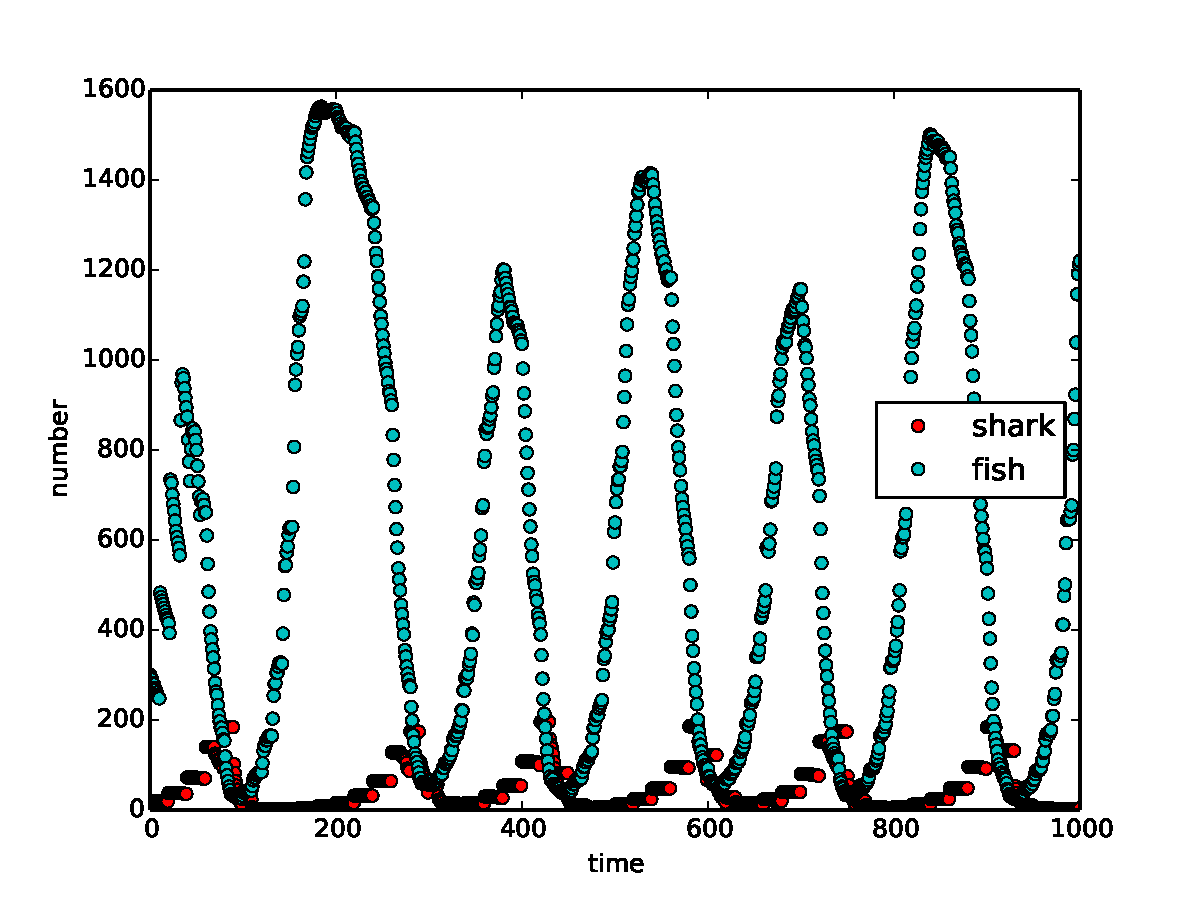
\includegraphics[width=10cm]{PP.pdf}
\caption{Numbers of fish and shark versus time. We see a quasi-periodic behaviour of predator and prey.}
\label{fig:graph}
\end{figure}
The behaviour of the populations are not regular; we see that the amplitude of the fish population in the plot is switches between a "higher" value (approximately 1400 to 1600 fish) and a "lower" value (approximately 1000 to 1200 fish) every other period. The shark population, on the other hand, exhibits a more regular amplitude, the peak of each period reaching approximately 200 sharks. This is interesting -- it seems that the sharks' maximum population is not noticeably dependent on the fish's maximum population. Moreover, the shark population's behaviour is sharper and less of a smooth curve; at each period, both the population and its first-order growth derivative increase until the curve hits a peak, after which both again decrease until the curve flattens out. The shark population reaches a peak at approximately the same relative time every period, which is at the point at which the fish population comes down from its peak and reaches 200 fish as well. We can see that the fish and shark populations, as they are coming down and going up respectively, both hit 200 and begin to decrease. The fish population begins to spike back up, and the shark population spikes up slightly after that. But, as expected, once the shark population is high, the fish begin to die off, which leads to the shark population dying off as well. This is the essence of the predator-prey model: if the prey population is high, the predator population thrives and increases as well, but once the number of predators increase, the number of prey decrease. This in turn causes the predators to die off, after which the prey begin to grow again -- all of which leads to the quasi-periodic model that is depicted in Figure \ref{fig:graph}.\par 
The initial parameters we used to reach this periodic behaviour in a 40 x 40 grid were: 300 initial fish, 20 initial sharks, 10 timesteps for the fish to breed, 20 timesteps for the shark to breed, and 10 timesteps for the shark to starve. So, the ratio between the initial numbers for the fish versus shark is 15:1, and the initial breeding ages for fish versus shark is 1:2. If the initial parameters stray too far from this value, either the sharks will go extinct first, and the fish will flood the grid, or the fish will go extinct first, causing the sharks to subsequently go extinct.\par
\bigskip
\noindent 2. \textbf{Snapshot configurations of our system}\par
Below is a link to a video of the shark-fish model, where the red squares are the fish and the blue squares are the sharks:\par
\href{https://github.com/LingfeiZhao/Group-Project-2b/blob/master/results/shark%20eat%20fish.mp4}{Video of shark-fish model}\par
We can see that the number of fish increase significantly before the number of sharks begin to noticeably increase -- the grid gets filled up with red squares before the increasing presence of blue squares eats away at the red ones. This is evident from Figure \ref{fig:graph} as well. It is also interesting to note that the video depicts how quickly sharks that have little to no surrounding fish die off, as we are able to observe entire regions of blue dots disappear in a single timestep. Another phenomenon that can be seen is that in some periods, the fish almost completely flood the grid before the shark population is able to catch up and eat the fish. While the maximum number of fish varies, as one can tell in the video, Figure \ref{fig:graph} tells us that the maximum number of sharks stays approximately the same. In some periods, the shark population is almost dangerously low; the at 0:15 and other snapshots, there are less than 7 sharks left in a grid of
40 x 40. However, we still observe multiple times that the shark population manages to rise despite that.\par
\bigskip
\noindent Github repository: \url{https://github.com/LingfeiZhao/Group-Project-2b}
\end{document}
